\documentclass[../Main.tex]{subfiles}
\begin{document}

\section{Introduction problems}

\subsection{Problem statement}

This is a website containing a large amount of information about houses and rooms that the owners do not currently need and want to rent out.
Visitors to the website can use search functions based on location, such as by city, district, or by specific address, like the house number on a particular street.
They can also search by rental price and the amenities of the houses or rooms available for rent.
The website provides detailed information about the houses or rooms available for rent, including the address and contact phone number for the landlord.

Instead of visiting each place to see rental properties, users only need an internet-connected device to access the website and search for the rental information they need, then contact the landlord.
The website also offers a real-time chat feature for users to conveniently exchange information.

\subsection{Purpose of this system}

\begin{itemize}
    \item User Interface: Design an intuitive interface that is easy to navigate and visually appealing.
    \item Basic Functionality: Implement essential features such as search functionality for finding rental information and an upload feature for landlords to post room details.
    \item Optimized Performance: Ensure the website is highly responsive by optimizing response times and loading speeds.
    \item Cost Efficiency: Minimize costs and distances for both landlords and tenants by efficiently connecting them through the platform.
    \item Admin Management: Provide an easy-to-use admin interface for managing room information and user interactions.
    \item Accurate Data Management: Ensure precise storage and retrieval of data to provide reliable information to users.
\end{itemize}

\section{Requirements Specification}

\subsection{Software Requirements Specification}

This document specifies the detailed requirements for a room rental web application, catering to administrators and customers.
The application aims to facilitate efficient room management and rental transactions.

\begin{table}[ht!]
    \caption{User Roles and Descriptions}
    \label{table:roles}
    \centering
    \begin{tblr}{|l|X|}
        \hline
        Role 1    & Descriptions \\
        \hline
        Admin     &
        Room and Pricing Management: Add, edit, and delete room types and pricing tiers.

        User Management: Manage user accounts, including CRUD operations.

        Confirmation of Uploaded Rooms: Review and approve rooms uploaded by landlords.

        Statistical Analysis: Generate reports on revenue, number of rooms in each region.
        \\
        \hline
        Customers &
        Search Functionality: Search for rooms based on room type, price range, area, etc.

        Registration and Login: Create an account and securely log in.

        Account Funding via Momo: Deposit funds into the account via Momo wallet to post more room listings.
        \\
        \hline
    \end{tblr}
\end{table}

\subsection{Functional Requirements Specification}

\subsubsection{Main Features of the Website}

Storage of Room Rental Information:
\begin{itemize}
    \item Store details about houses and rooms available for rent, such as location, address, rental price, and contact information for landlords.
    \item Ensure structured data storage for efficient and quick search functionality.
\end{itemize}
Attractive and User-Friendly Interface:
\begin{itemize}
    \item Design an appealing and user-friendly interface accessible to all user types.
\end{itemize}
Flexible Search Functionality:
\begin{itemize}
    \item Implement versatile search capabilities allowing users to quickly find rental information based on location, price range, and other relevant criteria.
\end{itemize}

\subsubsection{Users}

User Registration and Authentication:
\begin{itemize}
    \item Users can register for an account on the website.
          Upon successful registration, a confirmation code will be sent to the registered email address for verification.
    \item After successful verification, users can log in to the system using their credentials.
\end{itemize}

Flexible Room Search:
\begin{itemize}
    \item Users can search for rental properties based on various criteria such as price, location (address or region), room type, and area size.
\end{itemize}

Room Upload and Fee:
\begin{itemize}
    \item Users with authenticated accounts can upload room rental information.
          Each room upload will incur a fee of 10000 VND per submission.
\end{itemize}

Management of Uploaded Room Information:
\begin{itemize}
    \item Logged-in users can manage the details of rooms they have uploaded, including editing or deleting listings as needed.
\end{itemize}

\subsubsection{Admin}

User Management:
\begin{itemize}
    \item Admin can manage user accounts, including viewing user details and account statuses.
    \item Admin has the authority to suspend or deactivate user accounts if suspicious activities are detected.
\end{itemize}

Room Category Management:
\begin{itemize}
    \item Admin can add, edit, or delete room categories (types of rooms available for rent).
\end{itemize}

Post Management:
\begin{itemize}
    \item Admin can add, edit, or delete room listings posted by users.
\end{itemize}

Statistical Analysis:
\begin{itemize}
    \item Admin has access to statistical reports like revenue analysis and regional room count.
\end{itemize}

\subsection{Non-functional requirements specifications}

\subsubsection{Security}

\begin{itemize}
    \item Data validation: All input forms must undergo thorough validation to prevent incorrect or incomplete data storage, ensuring data integrity and reliability.
    \item User Access Control: Users who are not logged in should not have access to account details or room information associated with accounts.
    \item Data Encryption and Security: User account information, including passwords, must be encrypted and securely stored.
          Admins should not have access to view user passwords.
    \item Registration and Password Recovery Authentication: Registration and password recovery processes must include email verification using a code sent to the user's registered email address.
    \item Admin Access Control: Access to the admin dashboard and functionalities should be restricted to admin accounts only, ensuring proper authorization mechanisms are in place.
    \item API Security: All APIs must be authenticated using access tokens to prevent unauthorized access and ensure secure communication between client and server.
    \item User Revocation: User privileges should be revoked upon logout to ensure ongoing security and access control.
\end{itemize}

\subsubsection{Usability}

\begin{itemize}
    \item Simple and User-Friendly Interface: The interface should be straightforward and easy to use for all user demographics, ensuring a positive user experience.
    \item Scalability Under Load: The system should handle multiple users accessing it concurrently without significant performance degradation, ensuring robust performance during peak times.
    \item Fast Response Times: The system should respond quickly to user requests, minimizing wait times and providing a responsive user experience.
    \item Data Encryption and Theft Prevention: Critical data, especially user-sensitive information, must be encrypted to prevent theft and unauthorized access.
    \item Frontend and Backend Input Validation: Validate user inputs both at the frontend (client-side) and backend (server-side) to ensure data integrity and prevent malicious input.
    \item Separation of Admin and User Interfaces: Admin and user interfaces should be distinctly separated, with appropriate access controls and functionalities restricted to their respective roles.
\end{itemize}

\section{Entities relationships}

\subsection{Entities}

\subsubsection{Define all entities}

\begin{table}[H]
    \caption{Define all entities}
    \label{table:entities}
    \centering
    \begin{tblr}{|l|l|X|}
        \hline
        No & Entity         & Role                                                            \\
        \hline
        1  & Authority      & Describe the main roles of this website                         \\
        \hline
        2  & Blog           & Describe the rental house post                                  \\
        \hline
        3  & Category       & Categorize the objectives of each room on the website.          \\
        \hline
        4  & User           & Save and describe information of each user register account.    \\
        \hline
        5  & Contact        & Describe the information to contact to users                    \\
        \hline
        6  & Room           & Describe all information of each hostel.                        \\
        \hline
        7  & Status room    & Informing the owner about the validity of the room information. \\
        \hline
        8  & Image room     & Show images of this hostel to user can look at carefully.       \\
        \hline
        9  & Province       & Save all provinces in Vietnam.                                  \\
        \hline
        10 & Districts      & Save all districts of each province.                            \\
        \hline
        11 & Wards          & Save all wards of each district.                                \\
        \hline
        12 & History pay    & Save user payment information.                                  \\
        \hline
        13 & User-authority & Save role of each user.                                         \\
        \hline
    \end{tblr}
\end{table}

\subsubsection{Data of each entity}

\begin{table}[H]
    \caption{Table authority}
    \label{table:authority}
    \centering
    \begin{tblr}{|l|l|l|l|}
        \hline
        No & Field & Data type    & Description            \\
        \hline
        1  & Name  & Varchar(255) & Name of each authority \\
        \hline
    \end{tblr}
\end{table}

\begin{table}[H]
    \caption{Table Category}
    \label{table:category}
    \centering
    \begin{tblr}{|l|l|l|l|}
        \hline
        No & Field & Data type    & Description           \\
        \hline
        1  & ID    & Bigint(20)   & Primary key           \\
        \hline
        2  & Name  & Varchar(255) & Name of each category \\
        \hline
    \end{tblr}
\end{table}

\begin{table}[H]
    \caption{Table User}
    \label{table:user}
    \centering
    \begin{tblr}{|l|l|l|l|}
        \hline
        No & Field          & Data type    & Description                       \\
        \hline
        1  & ID             & Bigint(20)   & Primary key                       \\
        \hline
        2  & Activation-key & Varchar(255) & Status                            \\
        \hline
        3  & Actived        & Boolean      & Lock status                       \\
        \hline
        4  & Password       & Varchar(255) & Password to login                 \\
        \hline
        5  & Username       & Varchar(255) & Email to login                    \\
        \hline
        6  & Full name      & Varchar(255) & Name of users                     \\
        \hline
        7  & Phone          & Varchar(255) & Information to contact            \\
        \hline
        8  & Created-date   & Date         & The day created account           \\
        \hline
        9  & Created time   & Time         & The hours created account         \\
        \hline
        10 & Amount         & Double       & Money of accounts to post hostels \\
        \hline
        11 & Link-face      & Varchar(255) & Information to contact via FB     \\
        \hline
        12 & Avatar         & Varchar(255) & Present Image of each user        \\
        \hline
    \end{tblr}
\end{table}

\begin{table}[H]
    \caption{Table User-authority}
    \label{table:user-authority}
    \centering
    \begin{tblr}{|l|l|l|l|}
        \hline
        No & Field          & Data type    & Description                         \\
        \hline
        1  & User-ID        & Bigint(20)   & Sub key to link with table user     \\
        \hline
        2  & Authority name & Varchar(255) & Sub-key to link with table category \\
        \hline
    \end{tblr}
\end{table}

\begin{table}[H]
    \caption{Table blog}
    \label{table:blog}
    \centering
    \begin{tblr}{|l|l|l|X|}
        \hline
        No        & Field        & Data type            & Description                                   \\
        \hline
        1         & ID           & Bigint               & Primary key                                   \\
        \hline
        2 Content & Longtext     & Content of this blog                                                 \\
        \hline
        3         & Created-Date & Date                 & The date created this blog                    \\
        \hline
        4         & Created-Time & Time                 & The time created this blog                    \\
        \hline
        5         & Description  & Longtext             & Describe this blog                            \\
        \hline
        6         & Image banner & Varchar(255)         & Avatar                                        \\
        \hline
        7         & Title        & Varchar(255)         &                                               \\
        \hline
        8         & User\_ID     & Bigint               & Sub key to link with user who posts this blog \\
        \hline
        9         & Vi\_pham     & Boolean              & Status of blog                                \\
        \hline
    \end{tblr}
\end{table}

\begin{table}[H]
    \caption{Table Province}
    \centering
    \begin{tblr}{|l|l|l|X|}
        \hline
        No & Field & Data type   & Description                     \\
        \hline
        1  & ID    & Bigint      & Primary key                     \\
        \hline
        2  & Name  & Varchar(20) & Name of all province in Vietnam \\
        \hline
    \end{tblr}
\end{table}

\begin{table}[H]
    \caption{Table Districts}
    \centering
    \begin{tblr}{|l|l|l|X|} \hline
        No & Field        & Data type   & Description                         \\ \hline
        1  & ID           & Bigint      & Primary key                         \\ \hline
        2  & Name         & Varchar(20) & Name of all Districts in Vietnam    \\ \hline
        3  & Province\_ID & Bigint      & Sub-key to link with table province \\ \hline
    \end{tblr}
\end{table}

\begin{table}[H]
    \caption{Table Wards}
    \centering
    \begin{tblr}{|l|l|l|X|} \hline
        1 & ID            & Bigint      & Primary key                          \\ \hline
        2 & Name          & Varchar(20) & Name of all wards in Vietnam         \\ \hline
        3 & Districts\_ID & Bigint      & Sub-key to link with table districts \\ \hline
    \end{tblr}
\end{table}

\begin{table}[H]
    \caption{Table Room}
    \centering
    \begin{tblr}{|l|l|l|X|} \hline
        No & Field        & Data type    & Desciption                             \\ \hline
        1  & ID           & Bigint       & Primary key                            \\ \hline
        2  & Area         & Float        & Size of this room                      \\ \hline
        3  & Banner       & Varchar(255) & Avatar of this room                    \\ \hline
        4  & Created-date & Date         & The date to post this room             \\ \hline
        5  & Created-time & Time         & The time to post this room             \\ \hline
        6  & Description  & Longtext     & All important information of this room \\ \hline
        7  & Price        & Double       & The cost customer must pay a month     \\ \hline
        8  & Street       & Varchar      & Exactly location                       \\ \hline
        9  & Title room   & Varchar      & Title of this room to rent             \\ \hline
        10 & category\_id & bigint       & Sub-key to link with table category    \\ \hline
        11 & user\_id     & bigint       & Sub-key to link with table user        \\ \hline
        12 & ward\_id     & bigint       & Sub-key to link with table ward        \\ \hline
        13 & status\_room & bigint       & Sub-key to link with status\_room      \\ \hline
    \end{tblr}
\end{table}

\begin{table}[H]
    \caption{Table Image Room}
    \centering
    \begin{tblr}{|l|l|l|X|} \hline
        No & Field       & Data type    & Description                     \\ \hline
        1  & ID          & Bigint(20)   & Primary key                     \\ \hline
        2  & link\_image & varchar(255) & Link image to show this room    \\ \hline
        3  & room\_id    & Bigint       & Sub-key to link with table room \\ \hline
    \end{tblr}
\end{table}

\begin{table}[H]
    \caption{Table Status Room}
    \centering
    \begin{tblr}{|l|l|l|X|} \hline
        STT & Field & Data type    & Description         \\ \hline
        1   & Id    & Bigint(20)   & Primary key         \\ \hline
        2   & Name  & Varchar(255) & Status of this room \\ \hline
    \end{tblr}
\end{table}

\begin{table}[H]
    \caption{Table History-pay}
    \centering
    \begin{tblr}{|l|l|l|X|} \hline
        No & Field        & Data Type & Description               \\ \hline
        1  & ID           & Bigint    & Primary key               \\ \hline
        2  & Created Date & Date      & The date transaction      \\ \hline
        3  & Created Time & Time      & The time transaction      \\ \hline
        4  & Order-ID     & Varchar   & ID order online payment   \\ \hline
        5  & Request-ID   & Varchar   & ID request online payment \\ \hline
        6  & Total amount & Double    & Total money payment       \\ \hline
    \end{tblr}
\end{table}

\begin{table}[H]
    \caption{Table contact}
    \centering
    \begin{tblr}{|l|l|l|X|} \hline
        No & Field         & Data Type    & Description                                \\ \hline
        1  & ID            & Bigint       & Primary key                                \\ \hline
        2  & Content       & Varchar(255) & Content of this contact                    \\ \hline
        3  & Created\_date & date         & The date created contact                   \\ \hline
        4  & Created\_time & time         & The time created contact                   \\ \hline
        5  & da\_xem       & int          & Status if admin see contact or not         \\ \hline
        6  & Email         & varchar(255) & Information show this user created contact \\ \hline
        7  & Fullname      & varchar(255) & Name of user creating contact              \\ \hline
    \end{tblr}
\end{table}

\subsection{Relationship}

\begin{figure}[H]
    \centering
    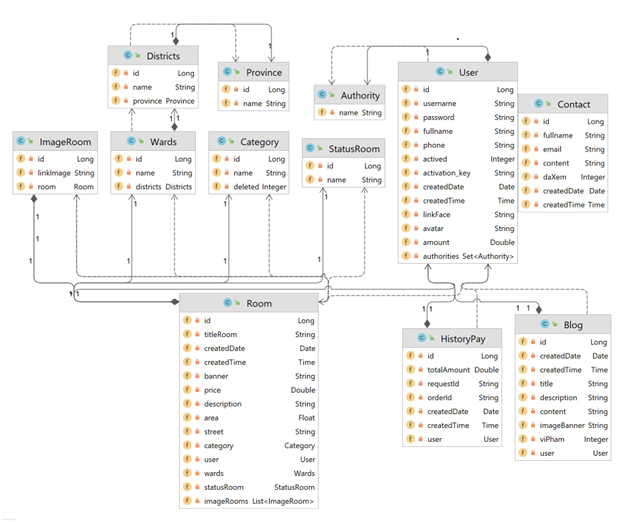
\includegraphics[width=\textwidth]{Figure/Picture7.png}
    \caption{Relationship}
    \label{fig:relationship}
\end{figure}

\section{Use cases diagram}

The use case diagram illustrates specific goals and how users interact with the system.
The ellipses within the system boundary represent the system's use cases or functions, while the stick figures symbolize the actors or users of the system.
The lines connecting the actors to the use cases indicate that the actors can perform those functions within the system to achieve their objectives.

\subsection{Use case general}

\begin{figure}[H]
    \centering
    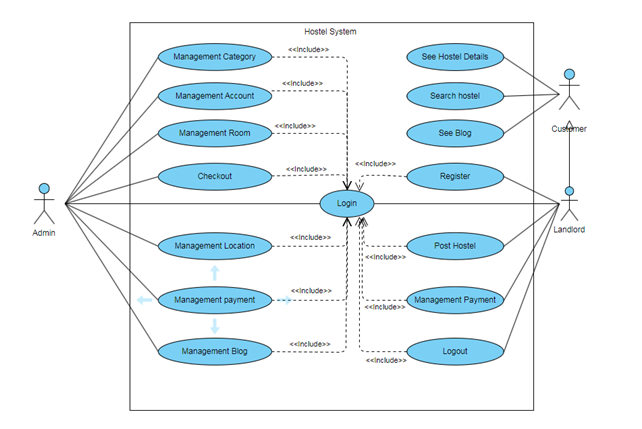
\includegraphics[width=\textwidth]{Figure/Picture8.png}
    \caption{Use case general}
    \label{fig:usecase}
\end{figure}

The website system comprises three main agents:
\subsubsection{Renter (or Tenant)}

Description: A user who directly interacts with the website's features such as viewing posts, searching for rental rooms, and accessing detailed room information.

Functions: View posts, search for rooms, view room details.

\subsubsection{Landlord}
Description: The user who posts room listings, with functions including managing posts, creating listings, depositing funds, logging in, and registering.

Functions: Manage posts, create listings, deposit funds, log in, register.

\subsubsection{Administrator}

Description: The role responsible for overseeing the entire system, including user management, post management, room category management, article management, and revenue management.

Functions: Manage users, manage posts, manage room categories, manage articles, manage revenue.

\subsection{Use case specifications}

\begin{enumerate}
    \item Use case view home page
          \begin{table}[H]
              \caption{Use case view home page}
              \centering
              \begin{tblr}{|l|X|} \hline
                  Objective      & This use case allows all people to see the home page                   \\ \hline
                  Actor          & Website visitors (Guest, User, Admin)                                  \\ \hline
                  Pre-condition  & The visitor must have internet access and a compatible web browser     \\ \hline
                  Main flow      &
                  1: The visitor navigates to the website's URL.

                  2: The system verifies if the visitor has an active session.

                  3: The system accesses the database to gather the required display information.

                  4: The system presents the homepage to the visitor.                                     \\ \hline
                  Post condition & The visitor is able to view the homepage and interact with its content \\ \hline
              \end{tblr}
          \end{table}
          Activities flow:
          \begin{figure}[H]
              \centering
              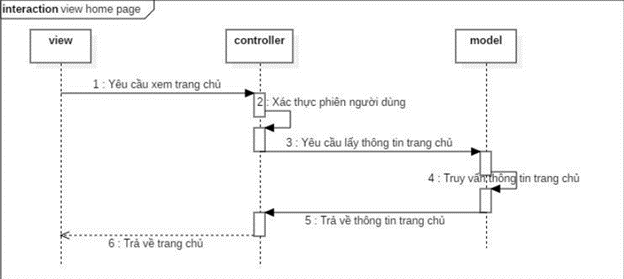
\includegraphics[width=\textwidth]{Figure/Picture9.png}
              \caption{Activities flow of UC view home page}
          \end{figure}

    \item Use case registration
          \begin{table}[H]
              \caption{Use case registration}
              \centering
              \begin{tblr}{|l|X|} \hline
                  Objective      & This use case allows all people to see the home page                   \\ \hline
                  Actor          & Website visitors (Guest, User, Admin)                                  \\ \hline
                  Pre-condition  & The visitor must have internet access and a compatible web browser     \\ \hline
                  Main flow      &
                  1: The visitor navigates to the website's URL.

                  2: The system verifies if the visitor has an active session.

                  3: The system accesses the database to gather the required display information.

                  4: The system presents the homepage to the visitor.                                     \\ \hline
                  Post condition & The visitor is able to view the homepage and interact with its content \\ \hline
              \end{tblr}
          \end{table}
          Activities flow:
          \begin{figure}[H]
              \centering
              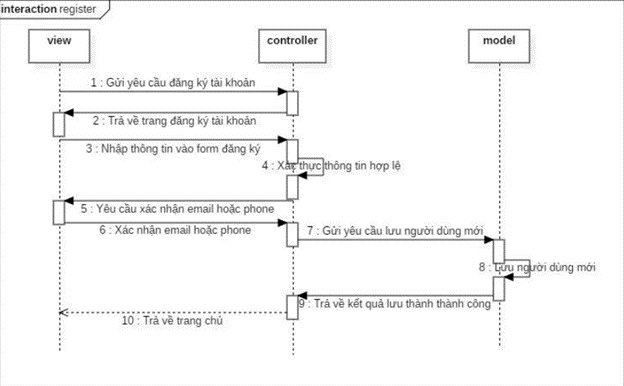
\includegraphics[width=\textwidth]{Figure/Picture10.png}
              \caption{Activities flow of UC registration}
          \end{figure}

    \item Use case search hostel
          \begin{table}[H]
              \caption{Use case search hostel}
              \centering
              \begin{tblr}{|l|X|} \hline
                  Objective      & This use case searches for hostels based on users’ requirements on the website .                         \\ \hline
                  Actor          & Potential guests looking for accommodation. (Guest, User, Admin)                                         \\ \hline
                  Pre-condition  & The user must have internet access and be on the hostel search                                           \\ \hline
                  Main flow      &
                  1: The user enters search criteria such as location, dates, area, and price.

                  2: The system processes the search query.

                  3: The system retrieves hostel information that matches the criteria from the database.

                  4: The system displays a list of hostels that meet the user’s requirements.

                  5: The system displays a list of hostels that meet the user’s requirements.                                               \\ \hline
                  Post condition & The user is presented with a list of hostels and can proceed to view more details or make a reservation. \\ \hline
              \end{tblr}
              \centering
          \end{table}
          Activites flows
          \begin{figure}[H]
              \centering
              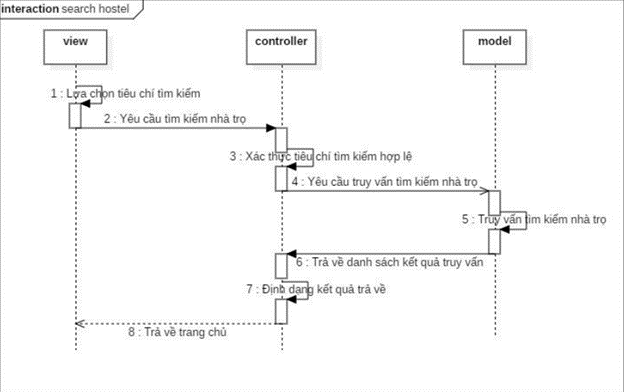
\includegraphics[width=\textwidth]{Figure/Picture11.png}
              \caption{ UC registration}
          \end{figure}

    \item Use case View hostel detail.
          \begin{table}[H]
              \centering
              \caption{Use case view hostel details}
              \begin{tblr}{|l|X|} \hline
                  Objective      & This use case allows all website’s visitors to view detailed information about a specific hostel on the website. \\ \hline
                  Actor          & Potential guests interested in hostel accommodations.                                                            \\ \hline
                  Pre-condition  & The user must have internet access and be on the website.                                                        \\ \hline
                  Main flow      &
                  1: The user selects a hostel from all hostels or the search results.

                  2: The system retrieves detailed information about the selected hostel from the database.

                  3: The system displays the detailed information, including photos, amenities, and pricing.                                        \\ \hline
                  Post condition & The user has access to comprehensive information about the hostel, which aids in making an informed decision.    \\ \hline
              \end{tblr}
          \end{table}
          Activities flow:
          \begin{figure}[H]
              \centering
              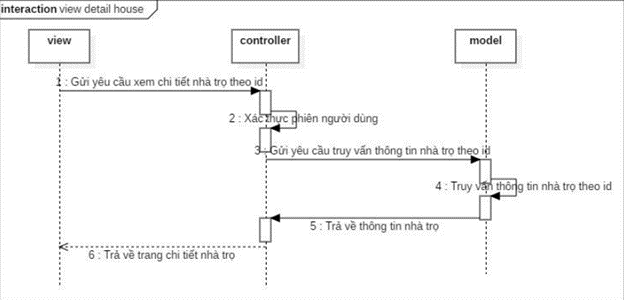
\includegraphics[width=\textwidth]{Figure/Picture12.png}
              \caption{ UC registration}
          \end{figure}

    \item Use case Login
          \begin{table}[H]
              \caption{Use case login to website}
              \centering
              \begin{tblr}{|l|X|} \hline
                  Objective      & This use case allows users to login to the website.                          \\ \hline
                  Actor          & Users                                                                        \\ \hline
                  Pre-condition  & The user must be registered and have valid login credentials.                \\ \hline
                  Main flow      &
                  1: The user navigates to the login page.

                  2: The user enters their username and password.

                  3: The system verifies the credentials.

                  \quad 3.1: If the credentials are wrong, the system will notice errors and return to the login page.

                  \quad 3.2: If the credentials are correct, the system grants access to the user’s account.

                  4: The user is redirected to the homepage or their dashboard.                                 \\ \hline
                  Post condition & The user is logged in and can access features available to registered users. \\ \hline
              \end{tblr}
          \end{table}
          Activities flow:
          \begin{figure}[H]
              \centering
              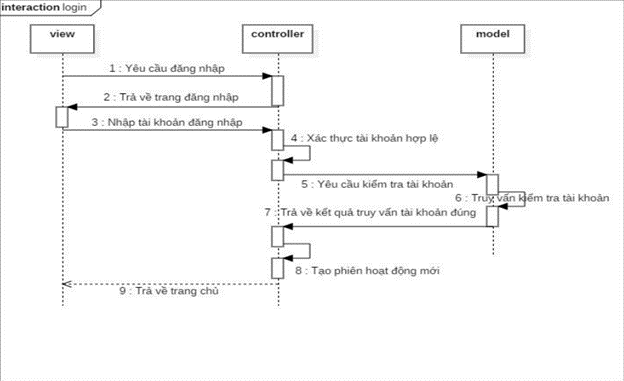
\includegraphics[width=\textwidth]{Figure/Picture13.png}
              \caption{ UC Login}
          \end{figure}

    \item Use case Restore password
          \begin{table}[H]
              \caption{Use case restore or reset password}
              \centering
              \begin{tblr}{|l|X|} \hline
                  Objective      & This use case allows users to restore or reset their password.                                              \\ \hline
                  Actor          & Users who have forgotten their password or wish to reset it.                                                \\ \hline
                  Pre-condition  & The user must have an existing account and access to the email or phone number associated with the account. \\ \hline
                  Main flow      &
                  1: The user clicks on the ‘Forgot Password’ or ‘Reset Password’ link.

                  2: The user enters their email address or phone number.

                  3: The system verifies the user’s information.

                  4: The system sends a password reset link or code to the user’s email or phone.

                  5: The user clicks on the reset link or enters the code provided.

                  6: The user sets a new password.                                                                                             \\ \hline
                  Post condition & The user has successfully reset their password and can now log in with the new credentials.                 \\ \hline
              \end{tblr}
          \end{table}
          Activities flow:
          \begin{figure}[H]
              \centering
              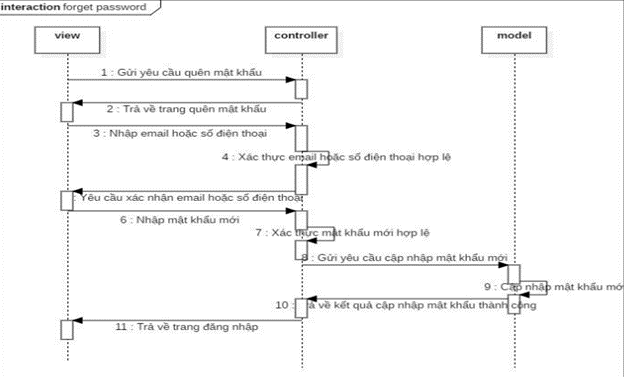
\includegraphics[width=\textwidth]{Figure/Picture14.png}
              \caption{ UC Restore password}
          \end{figure}

    \item Use case Post hostel.
          \begin{table}[H]
              \caption{Use case post a new blog for renting rooms or finding roommates}
              \centering
              \begin{tblr}{|l|X|} \hline
                  Objective      & This use case allows users to post a new blog to rent users’ room or find roommates.                  \\ \hline
                  Actor          & Hostels’ owner                                                                                        \\ \hline
                  Pre-condition  & The actor must be registered on the platform and have the necessary details and photos of the hostel. \\ \hline
                  Main flow      &
                  1: The owner/manager logs into their account.

                  2: They navigate to the ‘Post a Hostel’ section.

                  3: They enter details about the hostel, such as location, amenities, room types, and pricing.

                  4: They upload photos of the hostel.

                  5: They submit the hostel listing for review.

                  6: The system verifies the information and approves the listing.

                  7: The hostel is posted on the website and becomes visible to potential guests.                                        \\ \hline
                  Post condition & The hostel is successfully listed on the website and can be searched and booked by users.             \\ \hline
              \end{tblr}
          \end{table}
          Actitivies flow:
          \begin{figure}[H]
              \centering
              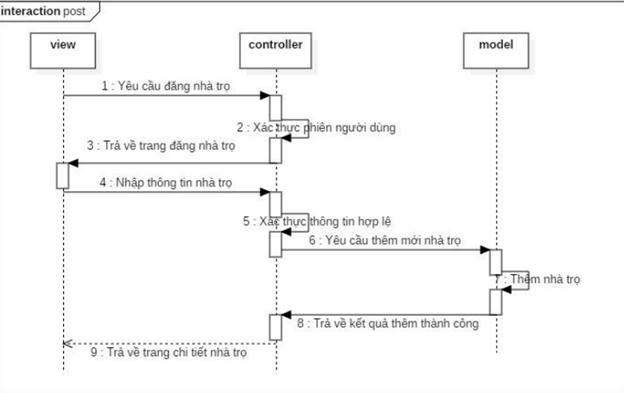
\includegraphics[width=\textwidth]{Figure/Picture15.png}
              \caption{ UC Post hostel}
          \end{figure}

    \item Use case view and update user information
          \begin{table}[H]
              \caption{Use case update user information}
              \centering
              \begin{tblr}{|l|X|} \hline
                  Objective      & This use case allows users to update their information on the website.                                            \\ \hline
                  Actor          & Users who want to change their information.                                                                       \\ \hline
                  Pre-condition  & The user must have internet access and be on the appropriate web page.                                            \\ \hline
                  Main flow      &
                  1: The user navigates to the section containing the information.

                  2: The user changes personal information in the fields they are able to change.

                  3: The user clicks on Update.

                  4: The system validates the new information.

                  \quad 4.1: If the new information is invalid, return to the view information page.

                  \quad 4.2: If the new information is valid, the system updates the information for the user.

                  5: The system notifies that the information has been updated successfully.                                                         \\ \hline
                  Post condition & The user’s information is updated in the system, and they can continue to use the website with their new details. \\ \hline
              \end{tblr}
          \end{table}
          Activities flow:
          \begin{figure}[H]
              \centering
              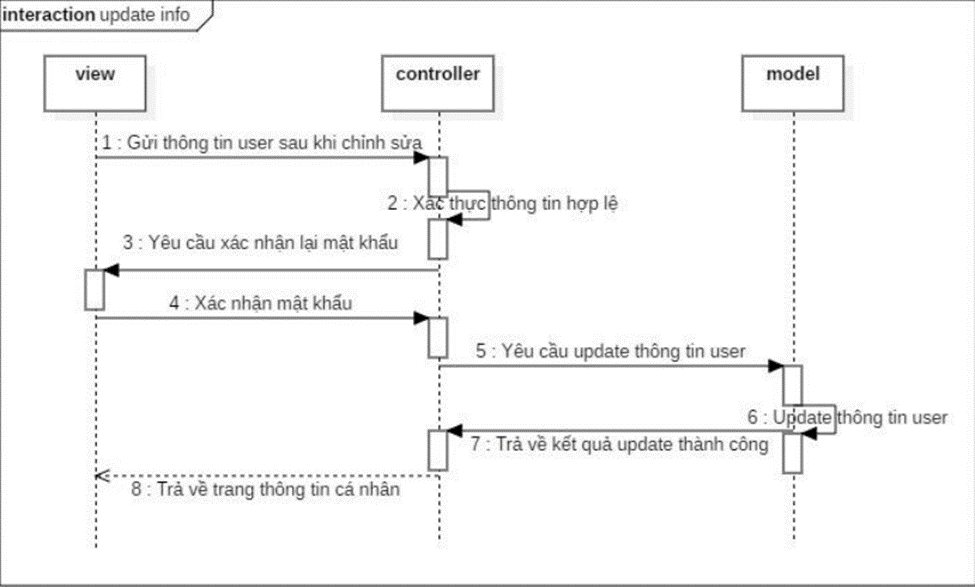
\includegraphics[width=\textwidth]{Figure/Picture16.png}
              \caption{ UC View and Update users information}
          \end{figure}

    \item Use case change passwords
          \begin{table}[H]
              \caption{Use case change password}
              \centering
              \begin{tblr}{|l|X|} \hline
                  Objective      & This use case allows users to change their password.                                            \\ \hline
                  Actor          & Users                                                                                           \\ \hline
                  Pre-condition  & The user must be logged in and have access to their account settings.                           \\ \hline
                  Main flow      &
                  1: The user navigates to the account settings or security settings page.

                  2: The user selects the option to change the password.

                  3: The user enters their current password for verification.

                  4: The user enters the new password and confirms it by entering it again.

                  5: The system validates the new password and updates the account credentials.

                  6: The system confirms the successful password change to the user.                                               \\ \hline
                  Post condition & The user’s password is updated, and they may be prompted to log in again with the new password. \\ \hline
              \end{tblr}
          \end{table}
          - Activities flow:
          \begin{figure}[H]
              \centering
              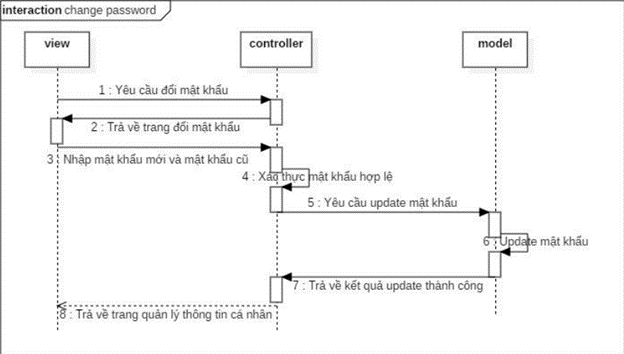
\includegraphics[width=\textwidth]{Figure/Picture17.png}
              \caption{ UC change password}
          \end{figure}

    \item Use case Update hostel information
          \begin{table}[H]
              \caption{Use case update property information}
              \centering
              \begin{tblr}{|l|X|} \hline
                  Objective      & This use case allows hostel owners or managers to update their property’s information on the website.               \\ \hline
                  Actor          & Hostel owners or managers.                                                                                          \\ \hline
                  Pre-condition  & The actor must be registered on the platform and have the necessary permissions to update the hostel’s information. \\ \hline
                  Main flow      &
                  1: The owner/manager logs into their account.

                  2: They navigate to the ‘My Hostels’ section.

                  3: They select the hostel whose information they wish to update.

                  4: They enter the updated information about the hostel, such as new amenities, updated pricing, or changes in availability.

                  5: They submit the updated information for review.

                  6: The system verifies the updated information and approves the changes.

                  7: The updated hostel information is posted on the website.                                                                          \\ \hline
                  Post condition & The hostel’s information is updated on the website, and potential guests can view the latest details.               \\ \hline
              \end{tblr}
          \end{table}
          Activities flow:
          \begin{figure}[H]
              \centering
              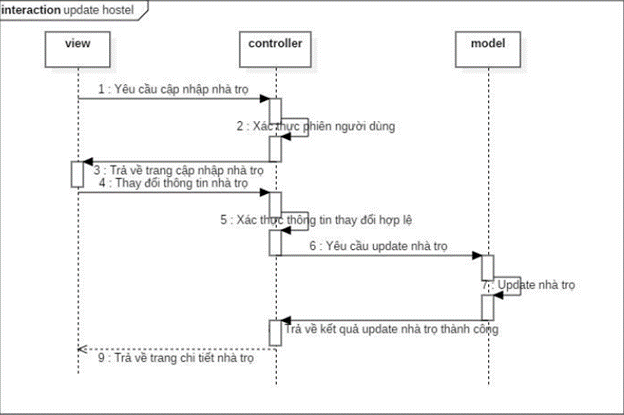
\includegraphics[width=\textwidth]{Figure/Picture18.png}
              \caption{ UC Update hostel information}
          \end{figure}

    \item Use case Delete hostel
          \begin{table}[H]
              \caption{Use case delete hostel listing}
              \centering
              \begin{tblr}{|l|X|} \hline
                  Objective      & This use case allows hostel owners or admin to delete or remove the hostel from the website.                        \\ \hline
                  Actor          & Hostel owners or Admin.                                                                                             \\ \hline
                  Pre-condition  & The actor must be registered on the platform and have the necessary permissions to delete the hostel’s information. \\ \hline
                  Main flow      &
                  1: The owner/manager logs into their account.

                  2: They navigate to the ‘My Hostels’ section.

                  3: They select the hostel listing they wish to delete.

                  4: They initiate the deletion process.

                  5: The system asks for confirmation to prevent accidental deletions.

                  6: Upon confirmation, the system removes the hostel listing from the website.                                                        \\ \hline
                  Post condition & The hostel listing is no longer available on the website, and users cannot search for or book it.                   \\ \hline
              \end{tblr}
          \end{table}
          Activities flow:
          \begin{figure}[H]
              \centering
              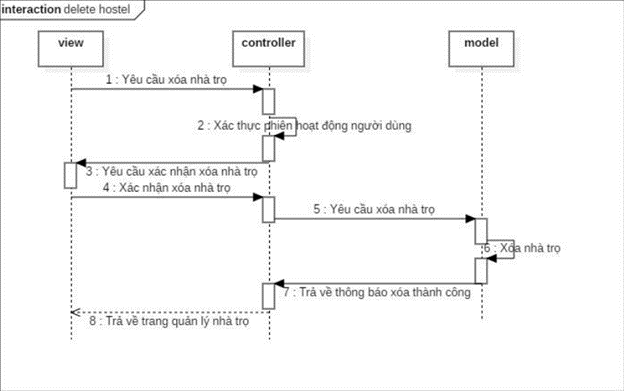
\includegraphics[width=\textwidth]{Figure/Picture19.png}
              \caption{ UC Delete hostel}
          \end{figure}

    \item Use case Logout
          \begin{table}[H]
              \caption{Use case logout from website}
              \centering
              \begin{tblr}{|l|X|} \hline
                  Objective      & This use case allows users or admins to logout from the website.                        \\ \hline
                  Actor          & Users, Admin                                                                            \\ \hline
                  Pre-condition  & The user must be logged in to the website.                                              \\ \hline
                  Main flow      &
                  1: The user clicks on the ‘Logout’ button or link.

                  2: The system ends the user’s session.

                  3: The user is redirected to the login page or the homepage of the website.                              \\ \hline
                  Post condition & The user is logged out and must log in again to access restricted areas of the website. \\ \hline
              \end{tblr}
          \end{table}
          Activities flow:
          \begin{figure}[H]
              \centering
              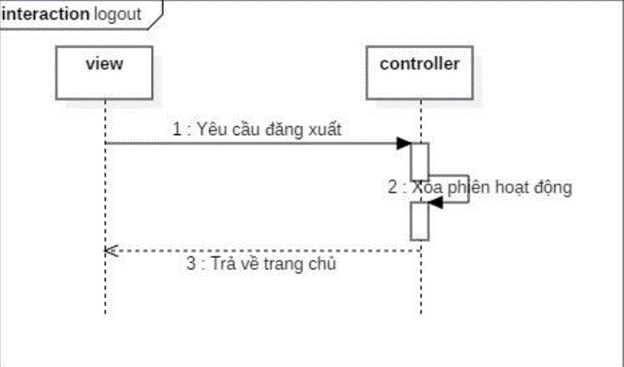
\includegraphics[width=\textwidth]{Figure/Picture20.png}
              \caption{ UC Logout}
          \end{figure}

    \item Use case delete user.
          \begin{table}[H]
              \caption{Use case remove user account}
              \centering
              \begin{tblr}{|l|X|} \hline
                  Objective      & This use case allows an administrator or authorized user to remove a user account from the system.    \\ \hline
                  Actor          & Admin                                                                                                 \\ \hline
                  Pre-condition  & The actor must be logged in with sufficient permissions to delete user accounts.                      \\ \hline
                  Main flow      &
                  1: The administrator navigates to the user management section.

                  2: They search for the user account they wish to delete.

                  3: They select the user account.

                  4: They initiate the deletion process.

                  5: The system asks for confirmation to prevent accidental deletions.

                  6: Upon confirmation, the system removes the user account from the system.

                  7: Both the user account and associated hostel listings are removed from the system.                                   \\ \hline
                  Post condition & The user account is no longer present in the system, and the user cannot log in or access the system. \\ \hline
              \end{tblr}
          \end{table}
          Activities flow:
          \begin{figure}[H]
              \centering
              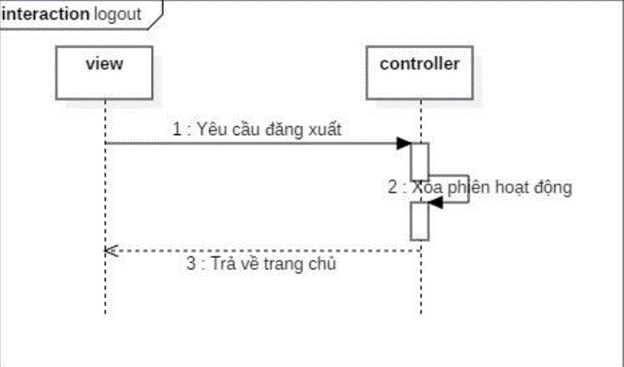
\includegraphics[width=\textwidth]{Figure/Picture20.png}
              \caption{ UC Logout}
          \end{figure}

    \item Use case Static
          \begin{table}[H]
              \caption{Use case analyze system's performance}
              \centering
              \begin{tblr}{|l|X|} \hline
                  Objective      & This use case allows an administrator to analyze the system’s work.                     \\ \hline
                  Actor          & Admin                                                                                   \\ \hline
                  Pre-condition  & Admin must be logged in.                                                                \\ \hline
                  Main flow      &
                  1: Admin clicks on “Analyze/Evaluate”.

                  2: The system redirects to the analysis page to evaluate the website's performance.

                  3: The system displays assessment charts about the website's performance.

                  \quad 3.1: Review analysis on Number of new users.

                  \quad 3.2: Analysis of reviews on Number of motels.

                  \quad 3.3: Analyzing and evaluating the distribution of boarding houses by area.                         \\ \hline
                  Post condition & The admin is able to view the report and analyze the data for decision-making purposes. \\ \hline
              \end{tblr}
          \end{table}

    \item Use case payment via Momo
          \begin{table}[H]
              \caption{Use case add money to user account via Momo}
              \centering
              \begin{tblr}{|l|X|} \hline
                  Objective      & This use case allows users to add money to their account via Momo to perform the post function.       \\ \hline
                  Actor          & User                                                                                                  \\ \hline
                  Pre-condition  &
                  User must be logged in.

                  User must have a valid payment method linked.
                  \\ \hline
                  Main flow      &
                  1: User selects the option to pay via Momo.

                  2: System redirects the user to the Momo payment gateway.

                  3: User confirms the payment amount and authorizes the transaction.

                  4: Momo processes the payment and deducts the specified amount from the user's Momo account.

                  5: Momo sends a payment confirmation or failure notification to the system.

                  \quad 5.1: If payment is successful, the system updates the user's account balance.

                  \quad 5.2: If the payment fails, Momo notifies the user and redirects back to the system without updating the balance. \\ \hline

                  Post condition &
                  User's account balance is increased by the amount added via Momo.

                  User can now use the balance to perform the post function.
                  \\ \hline
              \end{tblr}
          \end{table}
\end{enumerate}

\end{document}
